\chapter{Analýzy a návrh}\label{chap:AppSpecifications}

V minulých kapitolách byly popsány zásobníkové automaty a způsob jejich činnosti a jž existující aplikace. Tato kapitola už se bude věnovat samotné aplikaci, konkrétně její analýze a návrhu simulátoru.

\section{Analýza}

Cílem této práce je tedy vytvořit aplikaci, která uživateli umožní si graficky simulovat činnost jakéhokoliv zásobníkového automatu, deterministického i nedeterministického, přijímajícího prázdným zásobníkem nebo přijímacím stavem. Z důvodu lepší dostupnosti pro uživatele jsem se rozhodl zvolit webovou aplikaci, která bude dostupná všem uživatelům bez nutnosti stahování nebo instalace jakéhokoliv softwaru. 

Aplikace by měla uživateli poskytnou možnost nadefinovat si automat přímo v aplikace, k čemuž by měl sloužit formulář, nebo moct nahrát automat ze souboru. Oba způsoby zadávání automatu by měly provádět kontrolu, jestli automat neobsahuje nějakou chybu, např.~přechod obsahuje zásobníkový symbol, který není součástí zásobníkové abecedy. Dále si aplikace bude ukládat všechny zásobníkové automaty, aby se k nim mohl uživatel kdykoliv vrátit. Uživatel si bude moct zobrazit seznam všech uložených zásobníkových automatů, zobrazit si jejich definici, editovat je nebo je~smazat. Dále si bude moct automat stáhnout do souboru, aby ho mohl např.~sdílet s ostatními uživateli. 

Kterýkoliv z těch automatů si bude moct uživatel zobrazit v simulátoru. Simulátor bude zobrazovat vstupní pásku, zásobník a řídící jednotku, které budou vždy v aktuální konfigurace, a bude uživateli umožňovat pro jím zadaný vstup krokovat činnost automat s vyhodnocením, zda je slovo přijato nebo ne. Krokovat bude moct uživatel dopředu i dozadu, ručně nebo automaticky s časovým intervalem, jehož délka bude nastavitelná.

\section{Návrh stránky simulátoru}

Před samotnou implementací aplikace si bylo nutné uvědomit, co vše bude simulátor obsahovat za~prvky a jaké bude jejich rozložení. Návrh rozložení je na Obrázku~\ref{fig:SimulatorPageDesign}. Jako první jsem si navrhl rozložení vstupní pásky, zásobníku a řídící jednotky. --- na obrázku zakresleny modře. Dále potřebuji tlačítka na ovládání simulátoru --- pohyb dopředu a dozadu, zapnutí automatické simulace, zastavení a nastavení rychlosti. Ty jsou v oblasti v obrázku zakreslenou zeleně. Dále mi pak ještě chybí způsob, jak nastavit obsah vstupní pásky a ukončení simulátoru. K tomu slouží tlačítka v obrázku zakresleny červeně. Mezi ovládáním na levé straně a zásobníkem na pravé straně mi zůstalo spousta prázdného místa. To bude později využito na zobrazení definice aktuálního automatu nebo zobrazení historie již použitých přechodů.

\begin{figure}[h]
    \centering
    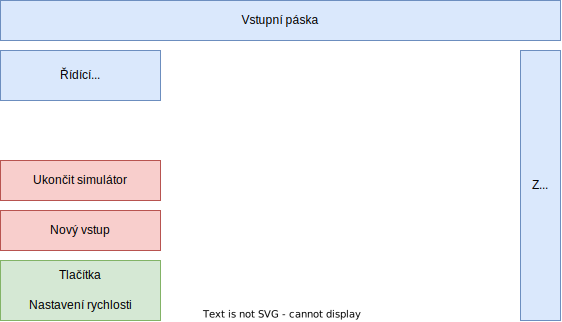
\includegraphics{Figures/SimulatoPageDesign.drawio.pdf}
    \caption{Návrh simulátoru}\label{fig:SimulatorPageDesign}
\end{figure}

\endinput